
\documentclass[conference]{IEEEtran}


% *** GRAPHICS RELATED PACKAGES ***
%
\ifCLASSINFOpdf
  % \usepackage[pdftex]{graphicx}
  % declare the path(s) where your graphic files are
  % \graphicspath{{../pdf/}{../jpeg/}}
  % and their extensions so you won't have to specify these with
  % every instance of \includegraphics
  % \DeclareGraphicsExtensions{.pdf,.jpeg,.png}
\else
  % or other class option (dvipsone, dvipdf, if not using dvips). graphicx
  % will default to the driver specified in the system graphics.cfg if no
  % driver is specified.
  % \usepackage[dvips]{graphicx}
  % declare the path(s) where your graphic files are
  % \graphicspath{{../eps/}}
  % and their extensions so you won't have to specify these with
  % every instance of \includegraphics
  % \DeclareGraphicsExtensions{.eps}
\fi
% graphicx was written by David Carlisle and Sebastian Rahtz. It is
% required if you want graphics, photos, etc. graphicx.sty is already
% installed on most LaTeX systems. The latest version and documentation
% can be obtained at: 
% http://www.ctan.org/pkg/graphicx
% Another good source of documentation is "Using Imported Graphics in
% LaTeX2e" by Keith Reckdahl which can be found at:
% http://www.ctan.org/pkg/epslatex
%
% latex, and pdflatex in dvi mode, support graphics in encapsulated
% postscript (.eps) format. pdflatex in pdf mode supports graphics
% in .pdf, .jpeg, .png and .mps (metapost) formats. Users should ensure
% that all non-photo figures use a vector format (.eps, .pdf, .mps) and
% not a bitmapped formats (.jpeg, .png). The IEEE frowns on bitmapped formats
% which can result in "jaggedy"/blurry rendering of lines and letters as
% well as large increases in file sizes.
%
% You can find documentation about the pdfTeX application at:
% http://www.tug.org/applications/pdftex



\usepackage{float}
\usepackage{subfigure}
\usepackage{amsmath}
\usepackage[textsize=tiny,textwidth=2cm]{todonotes}
\usepackage[ruled,vlined,linesnumbered]{algorithm2e}
\newcommand\mycommfont[1]{\footnotesize\ttfamily\textcolor{black}{#1}}
\SetCommentSty{mycommfont}
\usepackage{algpseudocode}
\usepackage{tikz}
\usetikzlibrary{shapes,arrows,positioning,calc}
\usepackage{url}

\newcommand\encircle[1]{%
  \tikz[baseline=(X.base)] 
    \node (X) [draw, shape=circle, inner sep=0] {\strut #1};}

% *** SUBFIGURE PACKAGES ***
%\ifCLASSOPTIONcompsoc
%  \usepackage[caption=false,font=normalsize,labelfont=sf,textfont=sf]{subfig}
%\else
%  \usepackage[caption=false,font=footnotesize]{subfig}
%\fi
% subfig.sty, written by Steven Douglas Cochran, is the modern replacement
% for subfigure.sty, the latter of which is no longer maintained and is
% incompatible with some LaTeX packages including fixltx2e. However,
% subfig.sty requires and automatically loads Axel Sommerfeldt's caption.sty
% which will override IEEEtran.cls' handling of captions and this will result
% in non-IEEE style figure/table captions. To prevent this problem, be sure
% and invoke subfig.sty's "caption=false" package option (available since
% subfig.sty version 1.3, 2005/06/28) as this is will preserve IEEEtran.cls
% handling of captions.
% Note that the Computer Society format requires a larger sans serif font
% than the serif footnote size font used in traditional IEEE formatting
% and thus the need to invoke different subfig.sty package options depending
% on whether compsoc mode has been enabled.
%
% The latest version and documentation of subfig.sty can be obtained at:
% http://www.ctan.org/pkg/subfig




% *** FLOAT PACKAGES ***
%
%\usepackage{fixltx2e}
% fixltx2e, the successor to the earlier fix2col.sty, was written by
% Frank Mittelbach and David Carlisle. This package corrects a few problems
% in the LaTeX2e kernel, the most notable of which is that in current
% LaTeX2e releases, the ordering of single and double column floats is not
% guaranteed to be preserved. Thus, an unpatched LaTeX2e can allow a
% single column figure to be placed prior to an earlier double column
% figure.
% Be aware that LaTeX2e kernels dated 2015 and later have fixltx2e.sty's
% corrections already built into the system in which case a warning will
% be issued if an attempt is made to load fixltx2e.sty as it is no longer
% needed.
% The latest version and documentation can be found at:
% http://www.ctan.org/pkg/fixltx2e


%\usepackage{stfloats}
% stfloats.sty was written by Sigitas Tolusis. This package gives LaTeX2e
% the ability to do double column floats at the bottom of the page as well
% as the top. (e.g., "\begin{figure*}[!b]" is not normally possible in
% LaTeX2e). It also provides a command:
%\fnbelowfloat
% to enable the placement of footnotes below bottom floats (the standard
% LaTeX2e kernel puts them above bottom floats). This is an invasive package
% which rewrites many portions of the LaTeX2e float routines. It may not work
% with other packages that modify the LaTeX2e float routines. The latest
% version and documentation can be obtained at:
% http://www.ctan.org/pkg/stfloats
% Do not use the stfloats baselinefloat ability as the IEEE does not allow
% \baselineskip to stretch. Authors submitting work to the IEEE should note
% that the IEEE rarely uses double column equations and that authors should try
% to avoid such use. Do not be tempted to use the cuted.sty or midfloat.sty
% packages (also by Sigitas Tolusis) as the IEEE does not format its papers in
% such ways.
% Do not attempt to use stfloats with fixltx2e as they are incompatible.
% Instead, use Morten Hogholm'a dblfloatfix which combines the features
% of both fixltx2e and stfloats:
%
% \usepackage{dblfloatfix}
% The latest version can be found at:
% http://www.ctan.org/pkg/dblfloatfix

\usepackage{url}
\hyphenation{op-tical net-works semi-conduc-tor}


\begin{document}
%
% paper title
% Titles are generally capitalized except for words such as a, an, and, as,
% at, but, by, for, in, nor, of, on, or, the, to and up, which are usually
% not capitalized unless they are the first or last word of the title.
% Linebreaks \\ can be used within to get better formatting as desired.
% Do not put math or special symbols in the title.
\title{GPaaScaler : Towards Green Energy Aware Scalable Cloud Platform}


% author names and affiliations
% use a multiple column layout for up to three different
% affiliations
\author{\IEEEauthorblockN{Sabbir Hasan}
\IEEEauthorblockA{INRIA\\
Nantes, France.\\
Email: sabbir.hasan@inria.fr}
\and

\IEEEauthorblockN{Frederico Alvares\\ and Thomas Ledoux}
\IEEEauthorblockA{IMT Atlantique\\
Nantes, France.\\
Email: firstname.lastname@inria.fr}
}

% conference papers do not typically use \thanks and this command
% is locked out in conference mode. If really needed, such as for
% the acknowledgment of grants, issue a \IEEEoverridecommandlockouts
% after \documentclass

% for over three affiliations, or if they all won't fit within the width
% of the page, use this alternative format:
% 
%\author{\IEEEauthorblockN{Michael Shell\IEEEauthorrefmark{1},
%Homer Simpson\IEEEauthorrefmark{2},
%James Kirk\IEEEauthorrefmark{3}, 
%Montgomery Scott\IEEEauthorrefmark{3} and
%Eldon Tyrell\IEEEauthorrefmark{4}}
%\IEEEauthorblockA{\IEEEauthorrefmark{1}School of Electrical and Computer Engineering\\
%Georgia Institute of Technology,
%Atlanta, Georgia 30332--0250\\ Email: see http://www.michaelshell.org/contact.html}
%\IEEEauthorblockA{\IEEEauthorrefmark{2}Twentieth Century Fox, Springfield, USA\\
%Email: homer@thesimpsons.com}
%\IEEEauthorblockA{\IEEEauthorrefmark{3}Starfleet Academy, San Francisco, California 96678-2391\\
%Telephone: (800) 555--1212, Fax: (888) 555--1212}
%\IEEEauthorblockA{\IEEEauthorrefmark{4}Tyrell Inc., 123 Replicant Street, Los Angeles, California 90210--4321}}





% make the title area
\maketitle

% As a general rule, do not put math, special symbols or citations
% in the abstract
\begin{abstract}
This chapter is an ongoing investigation on how to efficiently utilize the elasticity nature of the infrastructure resources when overall resource requirement of an application is higher than the existing underlying infrastructure can handle. Actions like adding/removing resource can be done independently at the infrastructure layer based on their utilization level \emph{i.e.,} cpu usage, memory usage etc. But, every application performs differently from one another at same cpu utilization level, specially when the resource utilization is medium to high. Therefore, coordinating the decision based on applications resource requirement or performance is the better way to devise scaling strategies. To this, firstly we propose to listen events from application to understand when to trigger scaling decision based on reactive and pro-active scaling rules. Secondly, we use traditional API such as \emph{scale-in} and \emph{scale-out} to trigger decision based on the strategy we have devised. Later we want to validate our approach by extensive experiments and results obtained over Grid'5000 test bed.
\end{abstract}

% no keywords

\IEEEpeerreviewmaketitle



\section{introduction}


The fast growth of internet technology and proliferation of Cloud services have multiplied data centers number in recent years. In 2016, data centers around the world consumed 416.2 TWh of electricity, which is significantly higher than the UK's total consumption of about 300 TWh on the same year\footnote{\url{http://www.independent.co.uk/environment/global-warming-data-centres-to \\-consume-three-times-as-much-energy-in-next-decade-experts-warn-a6830086.html}}. Although, numerous state-of-the-art energy efficient techniques have been adopted by industry and academia, a recent report suggests that energy usage in data centers is expected to increase by 4\% until 2020, which will translate to higher carbon emission. Most of today's data centers consume grid tied brown energy, very few are partially powered by renewable energy. Therefore, energy efficient techniques alone is not going to reduce the
carbon footprint since energy consumption will continue to grow.
On the other hand, the ever increasing enthusiasm and consciousness of reducing energy consumption can lead towards smarter ways to consume energy in cloud data centers. While an efficient energy management technique in data center can reduce unnecessary use of brown energy and better utilize green energy without going to waste \cite{parasol}, \cite{sabbir}, smarter ways of consuming energy in the presence/absence of renewable/green energy by an application can further reduce carbon footprint.

 

Traditionally, data centers host heterogeneous applications, such as \emph{interactive} and \emph{batch} applications/jobs. Goiri et al. \cite{GreenSlot}, \cite{GreenHadoop} first proposed a green energy adaptive framework for batch job oriented tasks \emph{i.e.,} that facilitated the scheduling of these tasks to different times by respecting the deadline when green energy is available. On the contrary, interactive
applications possess lesser flexibility, i.e., it should react with
little to no latency, otherwise Quality of Service (QoS) can
be seriously impacted. To cope up with these limitations, we have proposed a green energy adaptive solution to create green energy awareness inside the application that inherits the capability to smartly use the available green energy having \emph{static} amount of underlying resources \cite{cloudcom},\cite{tsc}.

But in a realistic cloud environment, resource requirement might exceed the currently provisioned resources. In contrast, when fewer resources are required, de-provisioning of resources can help to reduce unnecessary energy consumption. Therefore, the capability to detect when resources are required/dispensable and react to it so as to keep performance at a targeted level while energy consumption can be minimized is required. Taking application reconfiguration decision in isolation with resource scaling policies may lead to performance degradation and inconsistency to the system. Hence, coordination between two different types of elasticity (\emph{i.e.,} application reconfiguration vs infrastructure (de)provisioning) is necessary.

Most of the work in the literature propose: (i) multiple autonomic loops in a coordinated manner to control cluster level resources (\emph{i.e.,} one loop for controlling DVFS, another loop for deciding scaling actions)\cite{server-cluster}, \cite{shi}; (ii) per-application local manager which requests to a central autonomic manager to tune the number of cpu core, memory and to change the number of VM's \cite{morin1}, \cite{morin2}; (iii) adaptive framework to coordinate between system level (DVFS) and application level (degrading quality) adaptation to improve performance and power efficiency \cite{adaptcap}.

It is clearly visible that - synergy between application and infrastructure based on green energy availability is missing despite having elasticity capability in both layers. We believe that, integrating the autonomic logics of the infrastructure with the one in the applications is a important research direction.
Therefore, in response to the existing works, we propose a PaaS (Platform-as-a-Service) solution, named \emph{GPaaScaler} that inherits the capability to adapt both at \emph{application} and at \emph{infrastructure} level in facing to changing condition \emph{i.e.,} workload burst, performance degradation, quality of energy etc. We refer green energy to be better in quality, compared to brown energy.
Application adaptation is realized by dynamically re-configuring application's mode/service level on the fly based on performance and/or green energy availability, whereas infrastructure adaptation takes care of addition/removal of resources based on application's resource demand. During application adaptation, any dynamic change at the software layer that impacts the energy profile can be considered as switching to higher or lower modes/service levels.
To this point, we want to study the impact of application adaptation (based on the presence/absence of green energy) on infrastructure to have a global view of energy consumption incurred by the application.
Furthermore, both adaptation technique is built in separate modules and coordinated in a sequential manner. For example, when application's performance decreases due to heavy load, the PaaS solution first triggers adaptation to application by downgrading the functionality according to signed SLA (Service Level Agreement) and invokes resource requests to infrastructure module. Followed by the invocation requests, infrastructure adaptation module analyzes and decides whether resources are going to be added or the request is to be ignored. We have tested our proposal at Grid'5000 test bed with a real life application, workload and energy profile to show that, when green energy aware adaptation is adopted, around 35\% brown energy consumption can be reduced compared to a baseline approach. By reducing brown energy consumption, ratio of green energy to brown energy can be increased and subsequently carbon footprint can be appreciably reduced.
The rest of the paper is organized as follows. Section 2 describes the GPaaScaler architecture. In Section 3, several Application controllers and a generic Infrastructure controller are designed to investigate their impacts on energy consumption and QoS properties and Section 4 validate approach through extensive experiments. Furthermore, in Section 5, we provide discussion based on results and observation. Section 6 describes the related works and we conclude our work in Section 7.
\section{GPaaScaler architecture}

This section presents our auto-scaler architecture named \emph{GPaaScaler}, which continuously listens the instances of events \emph{e.g.,} response time, green energy availability, working modes of application etc., pushed by SaaS and IaaS in a changing environment. Furthermore, it inherits the capability to actuate both at application and at infrastructure level.
We use the most popular self-adaptive design framework: Monitor-Analyze-Plan-
Execute-Knowledge (MAPE-K) loop \cite{vision} for our auto-scaler.
Our contribution lies on the \emph{analyze} and \emph{plan} (A-P) block of this autonomic framework.

\begin{figure} [ht]
\centering
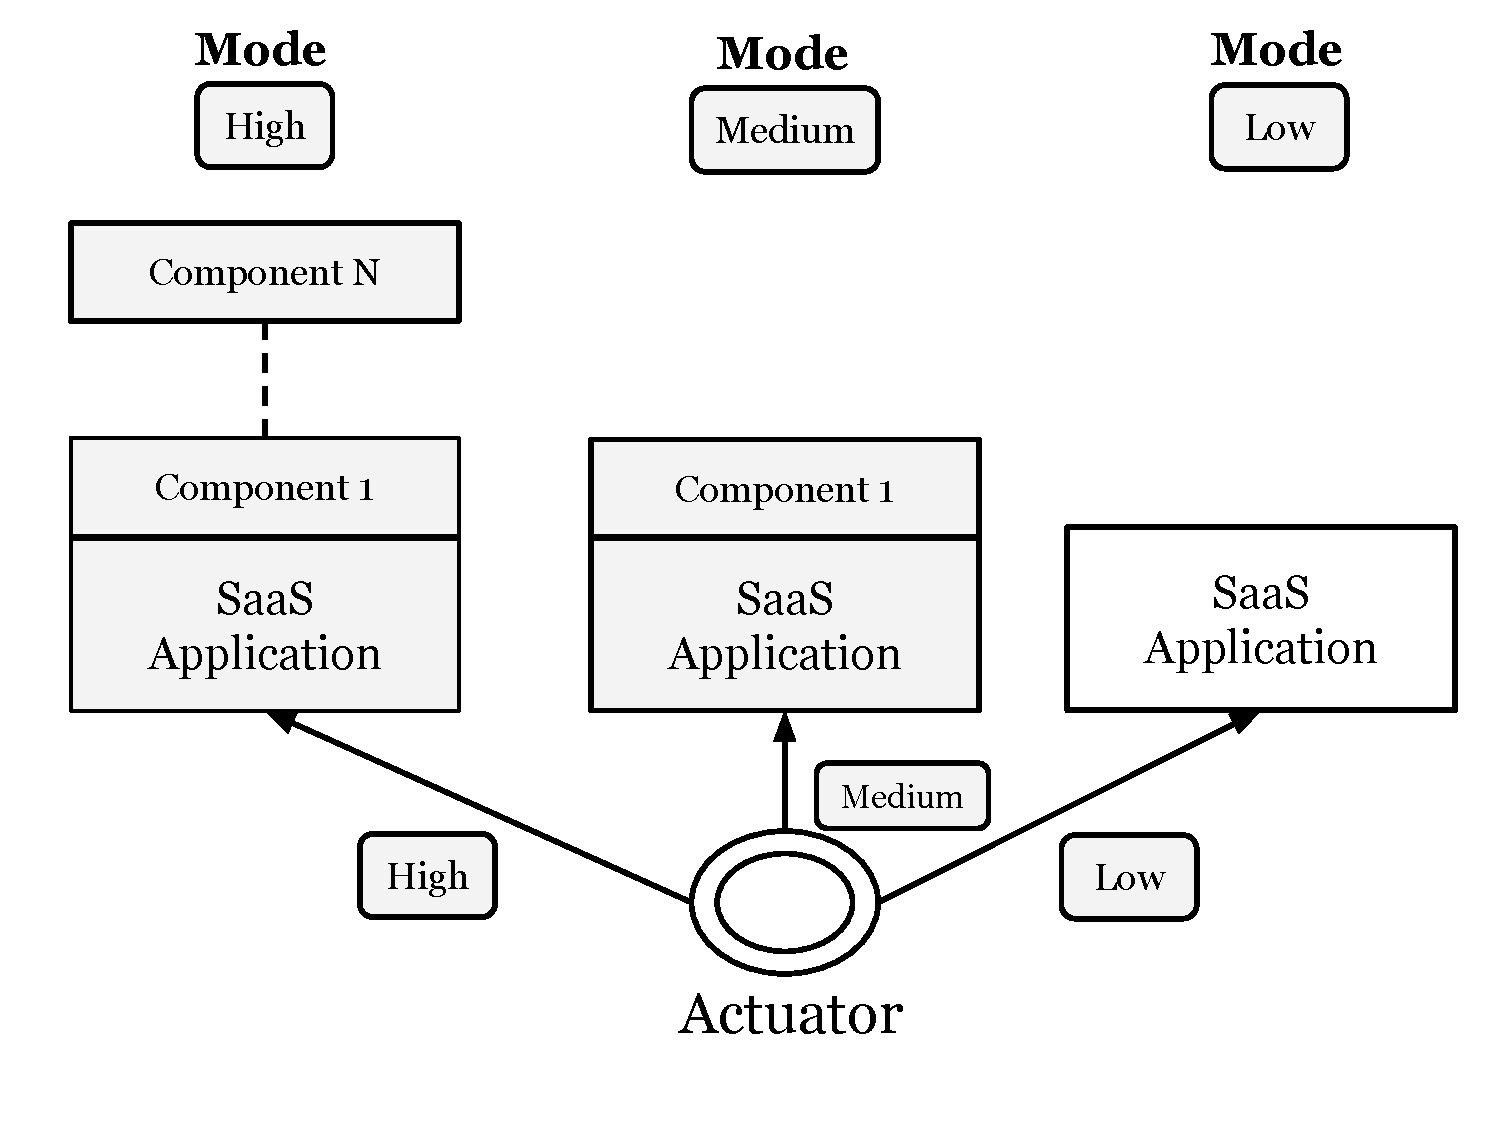
\includegraphics[scale=.32]{Graphs/action_1.pdf}
\caption{Applications mode under different service level}
\label{fig:modes}
\end{figure}

Monitoring (M) block pushes listened events to \emph{Analyze} block from SaaS layer (\emph{i.e.,} response time, workload, application's working mode, etc.) and IaaS layer (\emph{i.e.,} quality of energy). Analyze (A) block is responsible for analyzing and decoupling events to extract the pertinent information and feed appropriate event to the event handler at the SaaS controller. Once the configuration plan is ready, SaaS controller triggers action through SaaS actuator.
We propose three user experience levels. Mode High refers to high user
experience while Mode Medium and Mode Low indicate to medium and low user experience respectively (see Figure \ref{fig:modes}). When current application behavior deviates from target system state in terms of objective metrics, the auto-scaler gracefully downgrades the user experience from higher mode to lower mode and vice-versa through proper actuator value. Once SaaS actuator trigger the adaptation plan, it passes request for addition/removal of resources event as «RequestEvent» to IaaS controller if the former controller decides that application needs more/less resources, which is shown at Figure \ref{fig:GPaaScaler}. Following the event, IaaS controller decides to take action via traditional infrastructure API that is \emph{scale-in} and \emph{scale-out} or wait/discard the request issued by the SaaS controller. Therefore, the execution block is composed of two types of actuators, \emph{i.e.,} SaaS and IaaS actuator, which can be seen at Figure \ref{fig:GPaaScaler}. In addition, \encircle{1}, \encircle{2} and \encircle{3} depict the task flow of our auto-scaler, 
whereas, the sequential flow in an ordered way (from $1.a$ to $1.e$) is presented at the Figure \ref{fig:GPaaScaler} for highlighting the control flow of the event.
In summary, IaaS controller only gets activated if SaaS controller issues any «RequestEvent». However, our proposed IaaS controller are unware of resource allocation strategy, for instance, what types of VM is to be added/removed or in which server VM is to be located etc.  




\begin{figure} [ht]
\centering
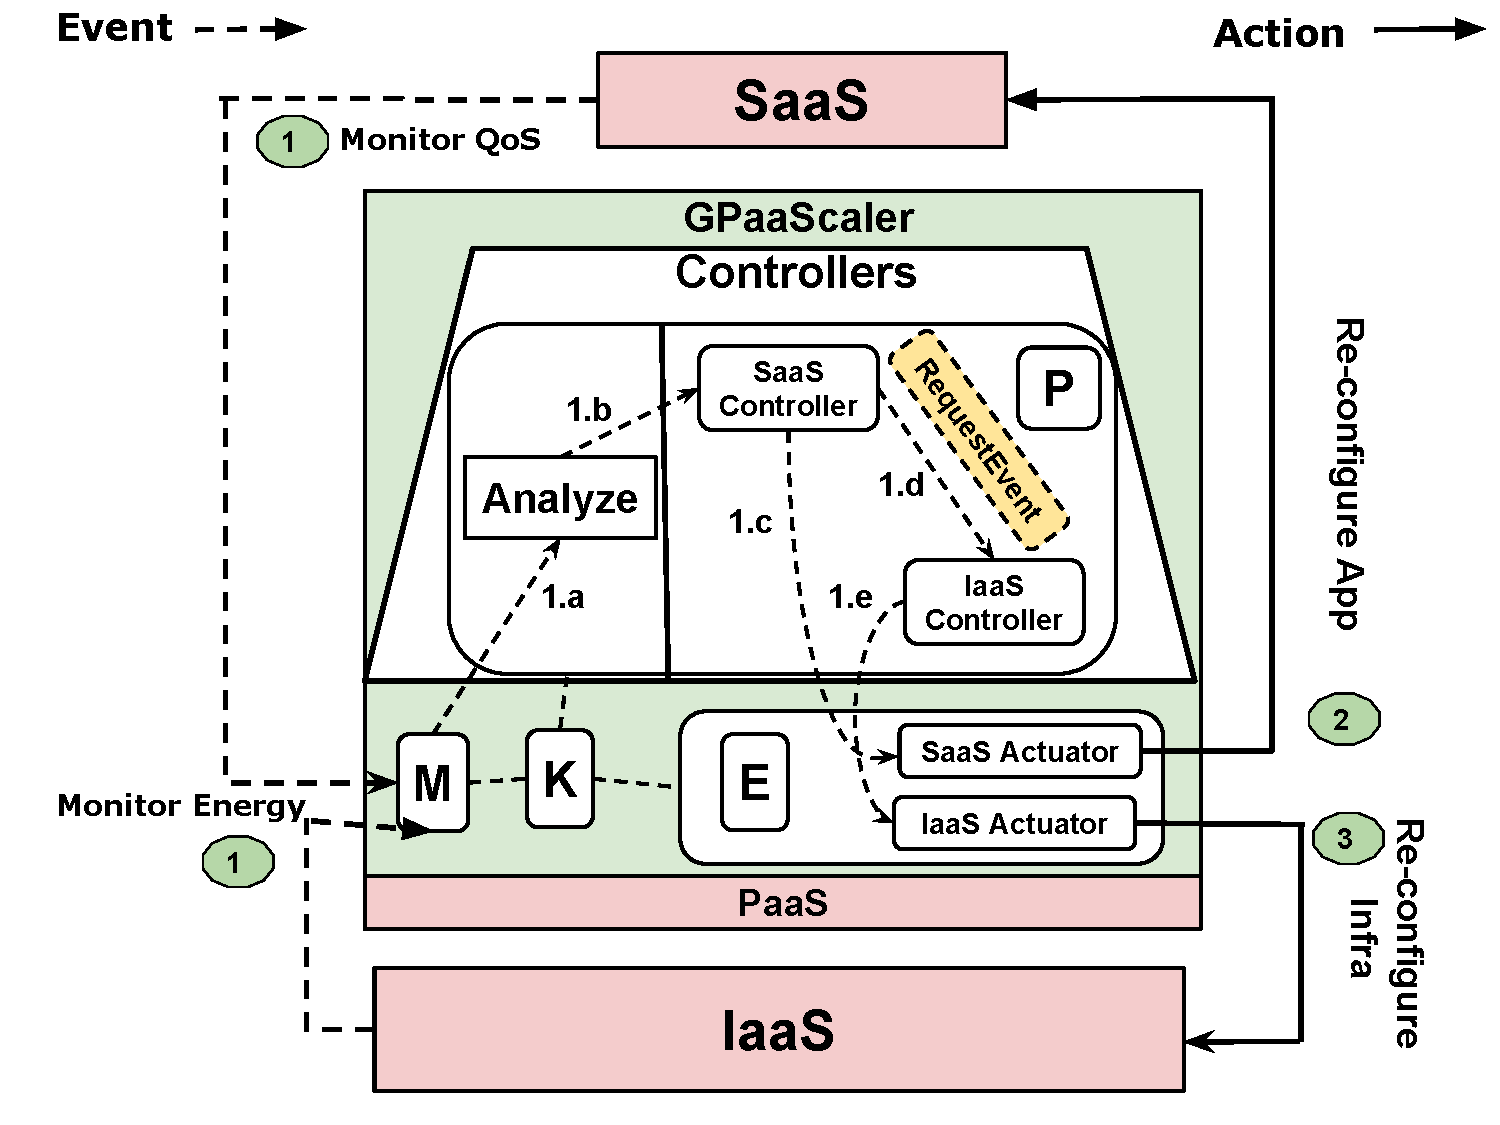
\includegraphics[scale=.38]{Graphs/test_gpaascaler.pdf}
\caption{GPaaScaler architecture}
\label{fig:GPaaScaler}
\end{figure}



\section{Proposed Controllers}

This section describes several application controllers which have been extended to leverage the underlying elastic infrastructure and a generic infrastructure controller which can be plugged with any application controller to control the elasticity capability of cloud infrastructure. 

\subsection{Application/SaaS controllers} \label{saas-controller}

% last chapter presents couple of controller. We choose the most performant one, and most energy efficient one with non-adaptive approach.

We have designed and validated several single and mutiple metric application controllers which have the capability to re-configure SaaS application to keep it accessible and performant even at changing conditions at \cite{sabbir},\cite{tsc}. In this article, we extend the Response time controller (performance aware) and Green Energy Controller (quality of resource aware) with increased capability to request of addition/removal of resources from the underlying elastic infrastructure.


\paragraph*{\textbf{Response Time controller (RT-C)}}
Response time is an essential metric to guarantee cloud
based application's performance. Our goal is to keep response
time under certain threshold dynamically to maximize the
availability of the service in unpredictable and variable
workload condition. We closed the managed software
system by a feedback loop, where in each control period, the
output is forwarded as a Map of response time and workload
arrival rate to compare with the target set-point. Afterwards, the information is forwarded to compute a function:

\begin{equation}
f(t)=1-\tilde{\lambda}(t)*\tilde{r}(t)
\end{equation} 

where \begin{math}\tilde{\lambda}(t) = \frac {\lambda(t-1)}
	{\lambda_{median}}\end{math} and \begin{math}\tilde{r}(t) =\frac
	{RT_{95}(t-1)} {RT_{setpoint}}\end{math}. Since,
unpredictability and burstiness of user requests is common phenomena for Cloud application, we have considered workload arrival rate $\lambda(t)$ as a disturbance to the system. Ignoring the disturbance can lead to dramatic degradation of application performance. For capturing the change in the workload
arrival rate, current workload arrival rate in the system is divided by median of
previous arrival rates. A median filter is used with window size of four, that provides better estimation about variability of the workload arrival rate. 
Furthermore, the function $f(t)$ is computed at each $t$ time to analyze how far the multiplication ratio of workload change and response time increment/decrement is from $1$. The idea is to keep the function greater than $0$ to stabilize
the system to operate under target response time. If the function is positive and above a desired/predefined threshold, the controller keeps the highest user experience mode \emph{i.e.,} mode 2. Since the controller is not aware of how much amount of underlying resources are used, it notifies the \emph{vmRemove} event to the IaaS controller (see line 13, Algorithm \ref{algo:rt_extended}). In case, the condition block falls to \emph{f(t) $\leq 0$}, a «RequestEvent» of \emph{vmAdd} is notified to IaaS controller (see line 10, Algorithm \ref{algo:rt_extended}).





%------------------------------Algorithm 2-------------------------
\begin{algorithm} [!ht]
\DontPrintSemicolon
\footnotesize
\KwIn { $Thr_{rt}, \lambda=[0 \quad 0 \quad 0 \quad 0], setPoint, app$ 
} 
\KwOut { updated $\lambda$, $Curr_{mode}$ = Current application mode. } 

\BlankLine 

\If {($handleEvent == responseTime$)}
     {    $\lambda(t-1)\gets servedRequest \ $ \;
         $enqueue(\lambda)$ \;
         $f(t)\gets 1-(\lambda(t-1)/\lambda_{median})*(RT_{95}/setPoint)$
	  
	   
		\If  { $(f(t) > 0) \enspace\land\enspace\  (function < Thr_{rt})$ } 
			     { $app.mode\gets mode \ 1$\;
			     $RequestEvent \rightarrow vmAdd$ \tcc*[f]{VM \emph{Addition} request event sent to IaaS controller along with $RT_{95}$ and workload-increment = $(\lambda(t-1)/\lambda_{median})$} \;}
		\ElseIf { $f(t) \leq 0$ } 
			{ $app.mode\gets mode \ 0$ \;
			$RequestEvent \rightarrow vmAdd$ \tcc*[f]{VM \emph{Addition} request event sent to IaaS controller along with $RT_{95}$ and workload-increment = $(\lambda(t-1)/\lambda_{median})$} \;}
 			\Else {$app.mode\gets mode \ 2$ \; 
 			       $RequestEvent \rightarrow vmRemove$ \tcc*[f]{VM \emph{Removal} request event sent to IaaS controller along with $RT_{95}$ and workload-increment = $(\lambda(t-1)/\lambda_{median})$} \;}
                $dequeue(\lambda)$ \; 
                $Curr_{mode} = app.mode$ \;			
 			
 			    							 							
 		}
\Return { $\lambda$, $Curr_{mode}$  } 
\caption {Response time controller (RT-C)} 
\label{algo:rt_extended}
\end{algorithm}
%--------------------------%End-%---------------------------------
 



\paragraph*{\textbf{Green Energy Controller (GE-C)}} While \emph{RT-C} is built to avoid performance degradation by keeping
response time to a target set point, is not aware of when green energy production is scarce or abundant to actuate application's mode. On the other hand, devising adaptation plan only based on green energy availability can dissatisfy reasonable QoS while workload arrival is higher.
Therefore, we intend to build a controller which can make adaptive decision based on the better quality of energy \emph{i.e.,} green energy and application's performance. 

We distinguish between two control periods: long and short. Algorithm \ref{algo:h_green_extended} presents two <<handleEvent>> blocks, each associated with specific event \emph{i.e.,} $greenEnergy$ and $responseTime$.
In \emph{longer control period}, $greenEnergy$ block decides application's mode based on green energy availability. Some sources of green energy are only available during certain times. For instance, solar energy is available during the day and the amount produced depends on the weather and the season \cite{GreenHadoop}. Due to the intermittency, we have divided the total green energy production to three different regions \emph{i.e.,} no green energy (at night), few (early morning and late afternoon) and adequate (mid-day). To distinguish between the regions we choose a static threshold $Thr_{max}$, above which the controller activates high user experience mode (mode 2). When green energy production falls between $0$ and $Thr_{max}$, the controller chooses an actuator value that triggers the medium user experience mode (mode 1), and in case of current green energy amount is null, mode 0 is activated. In short, the controller activates higher or lower user experience mode based on the energy information pushed by infrastructure in longer control periods. In contrast, the
$responseTime$ block checks the response time periodically in \emph{shorter control period} to identify overloaded condition in the system. If occurred,
the controller downgrades the user experience to lower level. In summary, depending on the event, the specific block gets activated in Algorithm \ref{algo:h_green_extended}.

Afterwards, we try to investigate when performance indicator of an Application can trigger add/remove VM request. Since this controller have two feedback loops activating at two different control periods: long and short, and longer control period's decision depends only on the energy information, hence we focus on the shorter control period loop which is based on response time event. The shorter control loop periodically checks if the targeted response time is violated by application by computing a function at line 15 at Algorithm \ref{algo:h_green_extended}. If the computed function becomes negative (f(t) $\leq 0$) meaning, if the current response time is beyond or borderline to set point and/or the tendency of the workload is increasing, the controller downgrades the user experience by subtracting 1 from previous control period's decision value and notify a \texttt{vmAdd} event request to the infrastructure controller (see line 18, Algorithm \ref{algo:h_green_extended}). While the function is greater than $0$, which suggests that the application is performing well by keeping current 95th percentile response time to the set point, application keeps the user experience as before but notify a \texttt{vmRemove} event request to the infrastructure controller (see line 21, Algorithm \ref{algo:h_green_extended}). In both cases, «RequestEvent» notifies the specific event along with application's current 95th percentile response time and workload increment ratio to the IaaS controller.

%------------- ALgorithm Green hybrid_extended -------------------------
\begin{algorithm} [!ht]
\DontPrintSemicolon
\footnotesize
\KwIn { $Thr_{max}$ = Threshold for green energy, $\lambda=[0 \quad 0 \quad 0 \quad 0]$, $setPoint$,$Curr_{GE}$ = Current green energy production. } 
\KwOut { updated $\lambda$, $Curr_{mode}$ = Current application mode.  } 

\BlankLine 
\emph{/* Initiates in longer control period */}\;

\If {($handleEvent == greenEnergy$)} 
{
\If  { $Curr_{GE} == 0$ } 
			     { $app.mode\gets mode \ 0$\;}
		\ElseIf { $Curr_{GE}>Thr_{max}$ } 
			{ $app.mode\gets mode \ 2$ \;}
 			\Else {$app.mode\gets mode \ 1$ \;}
 			      $Curr_{mode} = app.mode$ \;  
 			     }
\Return { $Curr_{mode}$ } 			      			   
\BlankLine  
\emph{/* Initiates in shorter control period */}\;  
  \If {($handleEvent == responseTime$)} 
     {    $\lambda(t-1)\gets servedRequest \ $ \;
         $enqueue(\lambda)$ \;
         $f(t) \gets 1-(\lambda(t-1)/\lambda_{median})*(RT_{95}/setPoint)$
	  
 \If { $(f(t) \leq0) \quad and  \quad (Curr_{mode} \neq0)$ }
			     { $app.mode\gets Curr_{mode}-1$ \;
			       $RequestEvent \rightarrow vmAdd$ \tcc*[f]{VM \emph{Addition} request event sent to IaaS controller along with $RT_{95}$ and workload-increment = $(\lambda(t-1)/\lambda_{median})$} \;}
 			\ElseIf {$(f(t)>0)$ }
 			{ $app.mode\gets Curr_{mode}$ \;
 			$RequestEvent \rightarrow vmRemove$ \tcc*[f]{VM \emph{Removal} request event sent to IaaS controller along with $RT_{95}$ and workload-increment = $(\lambda(t-1)/\lambda_{median})$} \;}
           
         \Else { $app.mode\gets Curr_{mode}$ \; }          			
             $Curr_{mode} = app.mode$\;
             $dequeue(\lambda)$ \;        			
           } 
              
\Return { $\lambda$, $Curr_{mode}$ } 
\caption {Green Energy controller (GE-C)}
\label{algo:h_green_extended}
\end{algorithm}






\subsection{IaaS controller}


While under-provisioning of resources can significantly hamper QoS properties by saturating application, over-provisioning of resources can increase energy consumption and other associated costs significantly. Therefore, the scaling decision, for instance, add resources (scale-out) or remove resources (scale-in) should be taken carefully to match with the applications resource demand. To meet \emph{scale-out} condition, a reactive policy can be easily designed and implemented based on the monitored performance metrics or by listening to predefined appropriate events. A reactive policy is referred to a runtime decision based on current demand and system state - to add resources on the fly. On the contrary, reactive policies can not absorb the non-negligible resource/instance initiation time. In our case, when application starts to face high response time, both the SaaS controllers have the capability to downgrade the user experience level and to invoke an implicit event (\texttt{vmAdd}) request to IaaS controller. Therefore, the sequential operation can trigger the application to run at lower mode until the instance is launched and activated. Afterwards, the application reverts back to higher mode if it meets the condition after operation.

In contrast, when \emph{scale-in} event (\emph{i.e.,} fewer resources are required by application) is invoked by SaaS controllers, terminating instance based on reactive policy can have detrimental impact on the system \cite{magali}. For example, when application performs better by staying just below or borderline to set point, triggering \emph{scale-in} action can make an application suffering from high response time to saturation. One way to overcome the problem is to VM resizing, that is to reduce the number of cpu cores on the fly by doing fine-grained analysis of resource requirements rather than terminating an entire instance, but popular hypervisors like KVM, VMware, Hyper-V does not allow removing cpu cores of guest VMs at runtime \cite{vertical}.
Additionally, instance termination can cause a sharp rise in response time reaching beyond the set point if workload's behavior or tendency is not taken into consideration. Therefore, devising a plan when to execute \emph{scale-in} event is critical. On the other hand, if the consecutive scaling actions are carried out too quickly without being able to observe the impact of scaling action to the application, undesirable effects such as over and under-provisioning can occur which can leads to performance degradation and/or wastage of energy consumption.
  
%------------- IaaS controller -------------------------
\begin{algorithm} [!ht]
\DontPrintSemicolon
\footnotesize
\KwIn { $[minVm , maxVm]$ = Minimum and maximum number of VM's. \\
$[RT_{95} , workload_{inc}]$ = Response time and workload increment sent by SaaS controller. \\
$[rt_{thr} , decWorkPerc]$ = Two tunable parameters.}
 
\KwOut { $vmNumber$, $coolingPeriod$ } 

\BlankLine 
%\emph{/* \textcolor{red}{Initiates in longer control period} */}\;

\If {($handleEvent == vmAdd$)} 
{
\If  { $(currentTime \notin coolingPeriod) \enspace \land \enspace(vmNumber < maxVm)$ } 
			     { $triggerAction \rightarrow "scale-out"$ \tcc*[f]{Passing API call through cloud infrastructure manager}\;
			       $vmNumber+=1$ \;
			       $coolingPeriod+=coolingLength$ \;
			       }
		
 			\Else {$vmNumber=this.vmNumber$ \;
 			       $coolingPeriod=this.coolingPeriod$ 
 			       }
 			       $vmNumber = update(vmNumber)$ \;  
 			       $coolingPeriod = update(coolingPeriod)$ \;
 }
 
\Return { $vmNumber$, $coolingPeriod$ } 			      			   
\BlankLine  
  
 \If {($handleEvent == vmRemove$)} 
 {
 \If  { $(currentTime \notin coolingPeriod) \enspace\land\enspace(rt_{thr} > RT_{95}) \enspace \land \enspace (vmNumber > minVm) \enspace \land \enspace ((workload_{inc} < decWorkPerc) \enspace \lor \enspace (Curr_{mode}=0))$ }
     
                   { $triggerAction \rightarrow "scale-in"$ \tcc*[f]{Passing API call through cloud infrastructure manager} \;
			       $vmNumber-=1$ \;
			       $coolingPeriod+=coolingLength$ \;
			       }
	  
                  \Else {$vmNumber=this.vmNumber$ \;
 			       $coolingPeriod=this.coolingPeriod$ \;
 			       }
 			       $vmNumber = update(vmNumber)$ \;  
 			       $coolingPeriod = update(coolingPeriod)$ \;
 }
 
\Return { $vmNumber$, $coolingPeriod$ } 
\caption {Infrastructure controller}
\label{algo:iaas_controller}
\end{algorithm}
%--------------------- END -----------------------------   

Hence, the idea is to built a generic IaaS controller which is characteristically agnostic to SaaS controllers behavior. Whenever, an implicit event invocation (\texttt{vmAdd, vmRemove}) arrives to the controller, it activates the proper module by matching to the event. Since, two non-concurrent events can be invoked by SaaS controllers, our proposed IaaS controller contains two modules to handle each of them. We define a length of period called \emph{coolingLength}, which is composed of instance activation time and the time it requires to impact on the application. Therefore, after triggering any scaling decision, this time period is updated to prevent any scaling decision to be made in between. Hence, when \texttt{vmAdd} event arrives to the controller, the $handleEvent == vmAdd$ module matches the condition of not being at $coolingPeriod$ with an and operator 
to maximum number of VM's a provider can be assigned to\footnote{Amazon EC2 permits maximum 20 on-demand instances per user.}. If it adheres the condition, \emph{scale-out} decision is triggered via IaaS actuator and current number of VM and next $coolingPeriod$ is updated (see line 3-5 of Algorithm \ref{algo:iaas_controller}). Otherwise, the module ignores the notification. On the other hand, when \texttt{vmRemove} event is invoked by SaaS controller, if the $handleEvent == vmRemove$ module is not carefully designed, cloud application can face unstable phases \emph{i.e.,} sharp rises of response time to saturate application. Therefore, only looking at $coolingPeriod$ and minimum number of VM
%\footnote{For a 3-tier application, at least one VM per tier should always run.}
 could be unwise and skeptical. 
 
To overcome this situation, we introduce two key parameters which are tunable to identify when is the good time to release resources \emph{i.e.,} perform scale-in action. The parameters are i) how far the current system's response time should be from set point? For example, x\% less than target response time set point, which is denoted by $rt_{thr}$ at Algorithm \ref{algo:iaas_controller}. ii) how much workload rate should decrease from the current trend? For instance, y\% decrease in user requests than previous intervals, denoted by \emph{decWorkPerc}. Hence, when $handleEvent == vmRemove$ arrives to the IaaS controller, the module checks the cooling period, minimum number of VM, current response time condition
with an AND operator. Additionally we put an OR operator between workload decrease parameter and current mode of the application. The rational behind that, in the absence of green energy, \emph{GE-C} controller keeps the application at minimum level. Although, workload may be consistent or increasing, if this application controller invokes \texttt{vmRemove} event that matches to be outside of $coolingPeriod$, greater than minimum number of VM and reduced response time than the threshold, it will meet the \emph{scale-in} condition and IaaS controller will trigger the action to release resources. On the other hand, \emph{RT-C} will keep application at the highest mode when resources are slightly to abundantly over-provisioned. Thus, application being at $mode=0$ and decreasing workload by y\% percentage can not happen concurrently if response time is x\% less than response time set point for this type of SaaS controller. Apart from \emph{GE-C}, any SaaS controller which invokes \texttt{vmRemove} event and satisfies all the conditions mentioned above other than application mode being at lowest, will trigger \emph{scale-in} action by IaaS controller.



%checks if the notification does not exist in coolingPeriod and if it exceeds the maximum amount of VM or not, if not it triggers scale-out action via IaaS actuator. 

%now dive into controller!



%\begin{thebibliography}{1}
%
%\bibitem{IEEEhowto:kopka}
%H.~Kopka and P.~W. Daly, \emph{A Guide to \LaTeX}, 3rd~ed.\hskip 1em plus
%  0.5em minus 0.4em\relax Harlow, England: Addison-Wesley, 1999.
%
%\end{thebibliography}




% that's all folks
\end{document}


